\documentclass[a4paper, xelatex, ja=standard]{bxjsarticle}
% \setpagelayout*{top=25truemm,bottom=25truemm,left=25truemm,right=25truemm}

% パッケージインストール
\usepackage{plisting}
\usepackage{docmute}

% 文書開始
\begin{document}
\maketitle
\begin{abstract}
Ray Tracing in One Weekend(週末レイトレーシング)
と言う書籍(サイト?)ではレイトレーシングをC++を使って
簡単に実装する方法について解説されている.
その中では当たり前だが多少の計算が必要で,
プログラミングやレイトレーシングに興味を持った未来の高専生たちが
いざ作ってみようと思っても(コード例が載っているので作ることはできるが)
完全に理解した状態で作るには説明が足りないと思われる.
そこでその計算方法やその他屈折に関する興味深い事実をまとめた.
\end{abstract}

\section{はじめに}
最近のゲームや映画の映像は
ものによっては現実と区別がつかないほど
高度な域にまで達している(特に金属や機械など).
商業的に使われているものほど細かいものは難しいが,
単純な金属球やガラス球といったものを
現実のような美しさで1から描画するのは
実はさほど難しくない.

レイトレーシングという3D CGの描画手法を使えば
(プログラミングを実行できる環境を持っていれば)
誰でも簡単に以下のような画像を生成させることができる.
\begin{figure}[b]
\centering
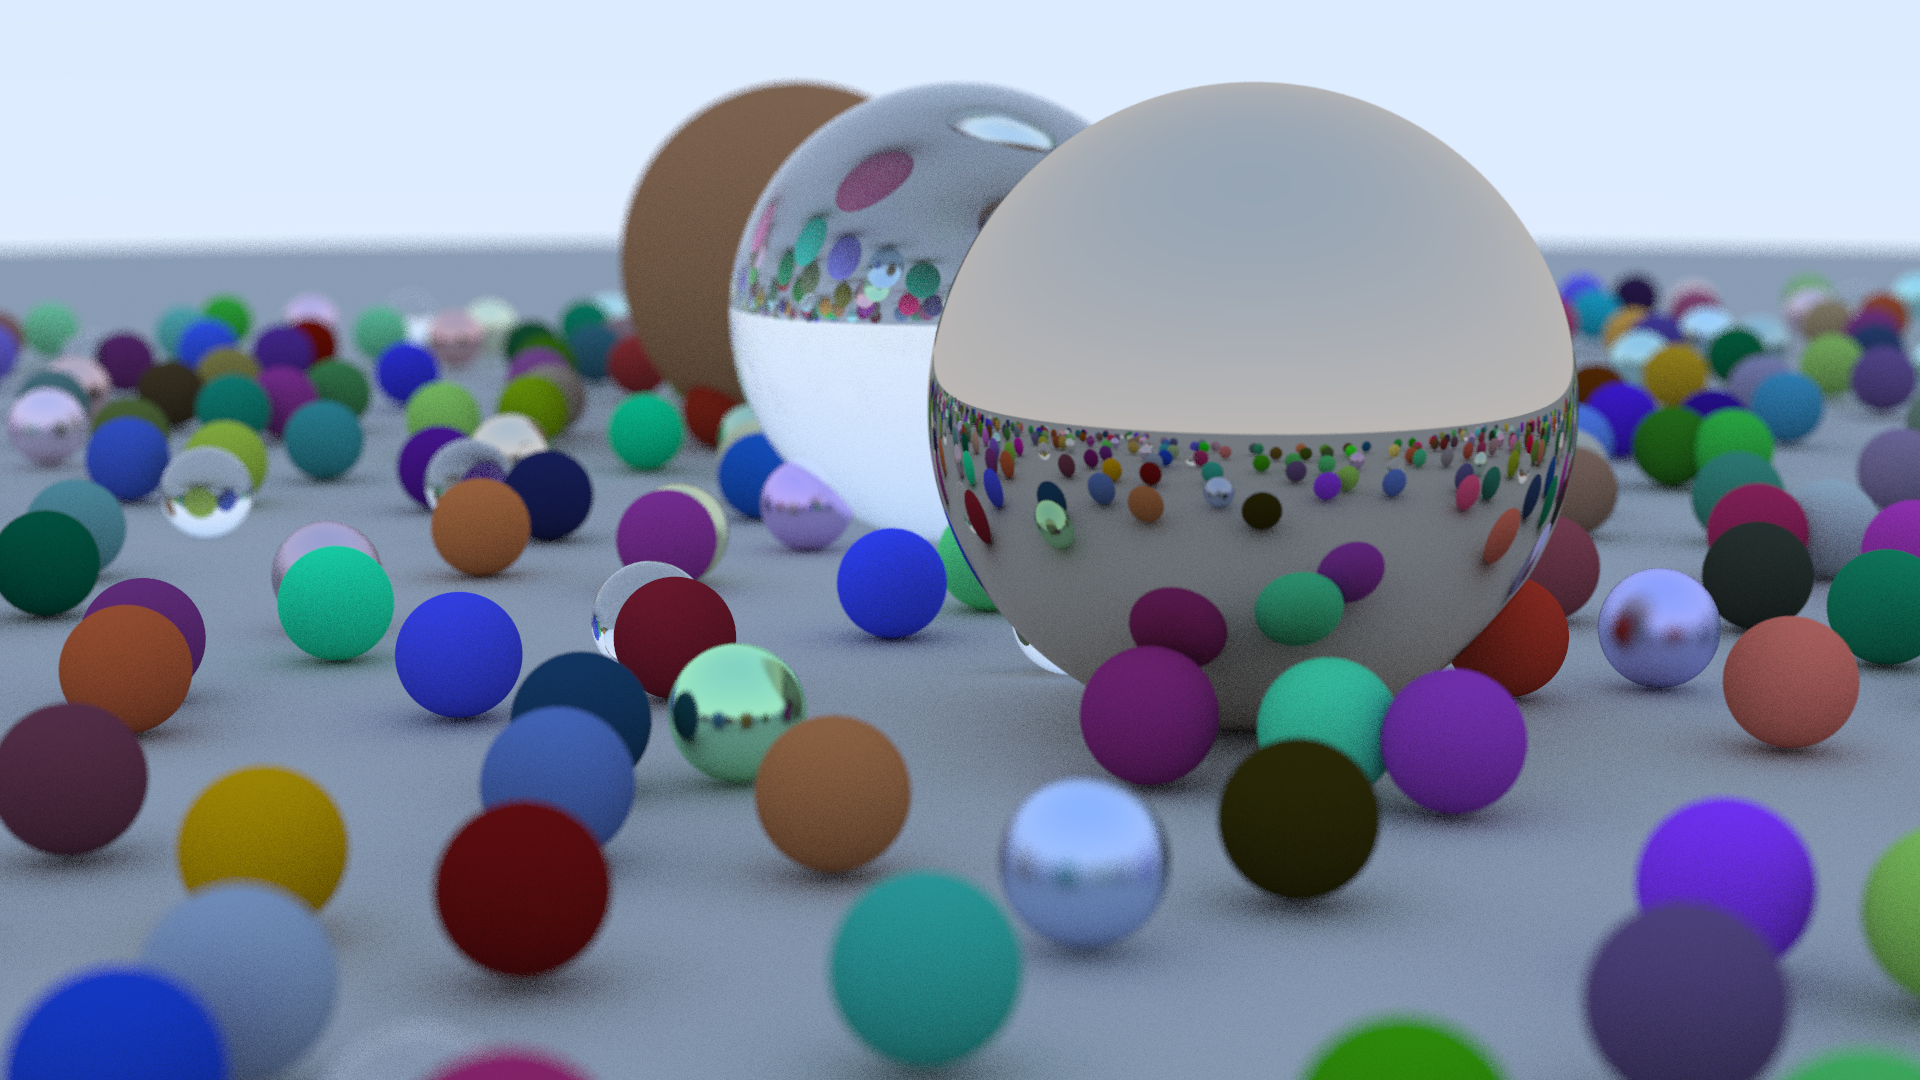
\includegraphics[scale=0.2]{img/example.png}
\caption{実際に描画した画像}
\label{}
\end{figure}
印刷の関係で白黒になっているだろうが
美しい画像を生成できることは確認できるだろう.
念を押すが誰でもBlenderやUnreal Engineといった
ソフトウェアを使わずに3D CGを描画できるのだ.

こちらではこれの作り方は説明しない.
既にRay Tracing in One Weekendという書籍(サイト?)
で作り方を無料公開しているからだ.
こちらではそのサイトでは説明不足に感じた
光の屈折の計算方法とそれに関する蛇足情報をまとめてある.

\section{光の屈折とは}
この宇宙で最速(量子もつれ\footnote{よくわかってないので自分で調べて}とかは無視)
の光くんは"真空中"で速度$c\simeq 300,000\si{km/s}$とされている.
これは1秒で地球を7周半できるほどの速さである
\footnote{速い, が宇宙の最速としては遅い, と思う}.
しかしこれは真空中の話で他の物質中(空気, 水, ガラス)を通っているときは
速度が落ちる.
光は粒子"でも"あるので実際に進むときは図 % あとでTikz追加して!!!
のように横1列になって進んでいると考えてほしい.

このように斜めに進んでいると
他の物質に入るのに時間差がうまれる.
この速度差と時間差が影響して
人の目からは光が他の物質へ入るときに
屈折するように見えるのだ.

ところで適当に流していたが, そもそもなぜ
「他の物質中(空気, 水, ガラス)を通っているときは速度が落ちる」
のだろう.

\section{屈折光の計算}
実際に屈折光をスネルの法則を中心に計算していくが
計算過程でいくつか高校数学で習うものを使う.
といってもちょろいので簡単な説明をしておく.

\subsection{必要になる知識の説明}
\subsubsection*{三角比}
\begin{center}
  	\begin{tikzpicture}[scale=2.25]
	    % \draw[->,>=stealth,semithick](-0.2,0)--(5,0)node[right]{$x$};% x軸
	    % \draw[->,>=stealth,semithick](0,-0.2)--(0,2)node[above]{$y$};% y軸
	    % \coordinate[label=below left:$\mathrm{O}$](O)at(0,0);%原点
	    % \coordinate(A)at(1,0);
	    % \coordinate(B)at(1.3,0);
	    % \coordinate(C)at(1.6,0);
	    % \coordinate(D)at(1.9,0);
	    % \coordinate(E)at(2.2,0);
	    % \coordinate(F)at(2.5,0);
	    % \coordinate(G)at(2.8,0);
	    % \coordinate(H)at(3.1,0);
	    % \coordinate(I)at(3.4,0);
	    % \coordinate(J)at(3.7,0);
	    % \coordinate(K)at(4,0);

	    \coordinate(A)at({sqrt(3)}, 1);
	    \coordinate(B)at(0, 0);
	    \coordinate(C)at({sqrt(3)}, 0);
	    
	    \draw(A)node[above]{$\mathrm{A}$};
	    \draw(B)node[left]{$\mathrm{B}$};
	    \draw(C)node[right]{$\mathrm{C}$};
	    
	    \draw(A)--(B)--(C)--(A);

	    % \draw plot[thick, domain=-0.2:4.5, smooth] (\x,{exp(-pow(\x/2-1, 2))+1/2});
	    % \fill[gray, opacity=0.3] (1,0) -- plot[domain=1:4, samples=100, smooth] (\x, {exp(-pow(\x/2-1, 2))+1/2}) -- (4,0);

	    % \draw[dashed](1, -0.2)--(1, 2)node[above]{$a$};
	    % \draw[dashed](4, -0.2)--(4, 2)node[above]{$b$};

	    % \draw(A)rectangle(1.3,{exp(-pow(1.3/2-1, 2))+1/2});
	    % \draw(B)rectangle(1.6,{exp(-pow(1.6/2-1, 2))+1/2});
	    % \draw(C)rectangle(1.9,{exp(-pow(1.9/2-1, 2))+1/2});
	    % \draw(D)rectangle(2.2,{exp(-pow(2.2/2-1, 2))+1/2});
	    % \draw(E)rectangle(2.5,{exp(-pow(2.5/2-1, 2))+1/2});
	    % \draw(F)rectangle(2.8,{exp(-pow(2.8/2-1, 2))+1/2});
	    % \draw(G)rectangle(3.1,{exp(-pow(3.1/2-1, 2))+1/2});
	    % \draw(H)rectangle(3.4,{exp(-pow(3.4/2-1, 2))+1/2});
	    % \draw(I)rectangle(3.7,{exp(-pow(3.7/2-1, 2))+1/2});
	    % \draw(J)rectangle(4,{exp(-pow(4/2-1, 2))+1/2});

	    % \draw(A)node[below left]{$x_0$};
	    % \draw(B)node[below]{$x_1$};
	    % \draw(C)node[below]{$x_2$};
	    % \draw(D)node[below]{$x_3$};
	    % \draw(E)node[below]{$x_4$};
	    % \draw(F)node[below]{$\cdots$};
	    % \draw(G)node[below]{$x_{k-1}$};
	    % \draw(H)node[below]{$x_k$};
	    % \draw(I)node[below]{$\cdots$};
	    % \draw(J)node[below]{$x_{n-1}$};
	    % \draw(K)node[below right]{$x_n$};

	    % \draw(4.5, {exp(-pow(4.5/2-1, 2))+1/2})node[right]{$f(x)$};

	    % \draw[looseness=1,bend left=60] (A) to node[above]{$\Delta x_1$}(B);
	    % \draw[looseness=1,bend left=60] (B) to node[above]{$\Delta x_2$}(C);
	    % \draw[looseness=1,bend left=60] (G) to node[above]{$\Delta x_k$}(H);
  	\end{tikzpicture}
\end{center}

図 % あとでTikz追加して!
のような直角三角形がある.
$\angle\mathrm{ABC}=\theta$とする.
それぞれ向かい合う辺を$a, b, c$とすると
三角比は以下のように定義される.
% \begin{align*}
% \sin{\theta}&=\frac{b}{c}\\
% \cos{\theta}&=\frac{a}{c}\\
% \tan{\theta}&=\frac{b}{a}
% \end{align*}
\[
\sin{\theta}=\frac{b}{c}\hspace{5mm}
\cos{\theta}=\frac{a}{c}\hspace{5mm}
\tan{\theta}=\frac{b}{a}
\]
なお今回使うのは$\sin$だけである.
また定義から明らかなことではあるが
斜辺の長さをかければそれぞれ高さ, 底辺の長さ
を求めることができる.

\subsubsection*{ベクトル}
今まで使ってきた長さや速さといったものは
1つの値で表してきた.
このようなものをスカラーと言う.
これに方向といった情報を追加し,
複数の値を使って表すものをベクトルという.
$\vec{a}$や$\vb{a}$などを使う.
今回は後者を使う. 格好良いから.
ベクトルの演算方法については,
加算, 内積, 大きさの計算方法がわかっていれば良いので, 
その3つについて説明する.

加算については図のようなイメージを持ってもらえば良い.
マイナスがついた場合方向が真逆になると思って欲しい.

内積は2つのベクトル$\vb{a, b}$のなす角を$\theta$とするとき
以下のように定義される.
\[
\vb{a}\cdot\vb{b}=|\vb{a}||\vb{b}|\cos{\theta}
\]
$|\vb{a}|$は$\vb{a}$の大きさを意味しており,
イメージとしては図の通りである.
式を見てもわかるが内積で得られる値はスカラーである.

\subsection{スネルの法則}

\subsection{全反射}

\subsection{フレネル反射率}

\section{最後に}
一番最初に紹介したのに最後に紹介するのは
あまり良くないかもしれないが,
最後にRay Tracing in One Weekendについて布教したいと思う.
そもそも

\begin{thebibliography}{9}
\bibitem{key1} Ray Tracing in One Weekend.
\end{thebibliography}

\end{document}